%%%%%%%%%%%%%%%%%%%%%%%%%%%%%%%%%%%%%%%%%%%%%%%%%%%%%%%%%%%%%%%%%%%%%%%%%%%%%%%%%%%%%%%%%%%%%%%%%%%%%%%%%%%%%%%%%%%%%%%%%%%%%%%%%%%%%%%%%%%%%%%%%%%%%%%%%%%%%%%%%%%
% Written By Michael Brodskiy
% Class: Circuits & Signals: Biomedical Applications
% Professor: N. Sun
%%%%%%%%%%%%%%%%%%%%%%%%%%%%%%%%%%%%%%%%%%%%%%%%%%%%%%%%%%%%%%%%%%%%%%%%%%%%%%%%%%%%%%%%%%%%%%%%%%%%%%%%%%%%%%%%%%%%%%%%%%%%%%%%%%%%%%%%%%%%%%%%%%%%%%%%%%%%%%%%%%%

\include{Includes.tex}

\title{Circuit Laws}
\date{\today}
\author{Michael Brodskiy\\ \small Professor: N. Sun}

\begin{document}

\maketitle

\begin{itemize}

  \item Voltmeter — Measures voltage without drawing current

  \item Ammeter — Measures current without dropping voltage

  \item Resistance is a function of size, shape, and media properties:

    $$\boxed{R=\frac{V}{I}=\frac{l}{\sigma A}=\rho\frac{l}{A}}$$

    \begin{itemize}

      \item $\sigma$ is the conductivity, $\rho$ is the resistivity, $l$ is the length of the wire, and $A$ is the cross-sectional area

    \end{itemize}

  \item Siemens (S), the unit for conductance, is the inverse of resistance, where: $\boxed{S=\dfrac{1}{\Omega}}$

    \begin{figure}[h!]
      \centering
      \tikzset{every picture/.style={line width=0.75pt}} %set default line width to 0.75pt        

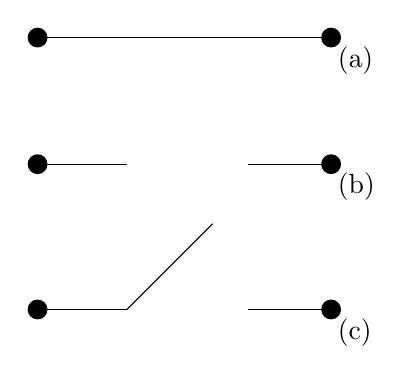
\begin{tikzpicture}[x=0.75pt,y=0.75pt,yscale=-1,xscale=1]
%uncomment if require: \path (0,359); %set diagram left start at 0, and has height of 359

%Shape: Boxed Line [id:dp6814534710440301] 
\draw    (399.71,51) -- (258.29,51) ;
%Shape: Circle [id:dp916629887844314] 
\draw  [fill={rgb, 255:red, 0; green, 0; blue, 0 }  ,fill opacity=1 ] (262.79,51) .. controls (262.79,48.51) and (260.77,46.5) .. (258.29,46.5) .. controls (255.8,46.5) and (253.79,48.51) .. (253.79,51) .. controls (253.79,53.49) and (255.8,55.5) .. (258.29,55.5) .. controls (260.77,55.5) and (262.79,53.49) .. (262.79,51) -- cycle ;
%Shape: Circle [id:dp26516064705603304] 
\draw  [fill={rgb, 255:red, 0; green, 0; blue, 0 }  ,fill opacity=1 ] (404.21,51) .. controls (404.21,48.51) and (402.2,46.5) .. (399.71,46.5) .. controls (397.23,46.5) and (395.21,48.51) .. (395.21,51) .. controls (395.21,53.49) and (397.23,55.5) .. (399.71,55.5) .. controls (402.2,55.5) and (404.21,53.49) .. (404.21,51) -- cycle ;
%Shape: Boxed Line [id:dp10516732114391769] 
\draw    (399.71,112) -- (258.29,112) ;
%Shape: Circle [id:dp05809513039601466] 
\draw  [fill={rgb, 255:red, 0; green, 0; blue, 0 }  ,fill opacity=1 ] (262.79,112) .. controls (262.79,109.51) and (260.77,107.5) .. (258.29,107.5) .. controls (255.8,107.5) and (253.79,109.51) .. (253.79,112) .. controls (253.79,114.49) and (255.8,116.5) .. (258.29,116.5) .. controls (260.77,116.5) and (262.79,114.49) .. (262.79,112) -- cycle ;
%Shape: Circle [id:dp7509947812401938] 
\draw  [fill={rgb, 255:red, 0; green, 0; blue, 0 }  ,fill opacity=1 ] (404.21,112) .. controls (404.21,109.51) and (402.2,107.5) .. (399.71,107.5) .. controls (397.23,107.5) and (395.21,109.51) .. (395.21,112) .. controls (395.21,114.49) and (397.23,116.5) .. (399.71,116.5) .. controls (402.2,116.5) and (404.21,114.49) .. (404.21,112) -- cycle ;
%Straight Lines [id:da01088402519767695] 
\draw [color={rgb, 255:red, 255; green, 255; blue, 255 }  ,draw opacity=1 ][fill={rgb, 255:red, 255; green, 255; blue, 255 }  ,fill opacity=1 ]   (301.29,112) -- (359.71,112) ;
%Shape: Boxed Line [id:dp9035438017815973] 
\draw    (399.71,182) -- (258.29,182) ;
%Shape: Circle [id:dp6675627274341545] 
\draw  [fill={rgb, 255:red, 0; green, 0; blue, 0 }  ,fill opacity=1 ] (262.79,182) .. controls (262.79,179.51) and (260.77,177.5) .. (258.29,177.5) .. controls (255.8,177.5) and (253.79,179.51) .. (253.79,182) .. controls (253.79,184.49) and (255.8,186.5) .. (258.29,186.5) .. controls (260.77,186.5) and (262.79,184.49) .. (262.79,182) -- cycle ;
%Shape: Circle [id:dp4832675708977021] 
\draw  [fill={rgb, 255:red, 0; green, 0; blue, 0 }  ,fill opacity=1 ] (404.21,182) .. controls (404.21,179.51) and (402.2,177.5) .. (399.71,177.5) .. controls (397.23,177.5) and (395.21,179.51) .. (395.21,182) .. controls (395.21,184.49) and (397.23,186.5) .. (399.71,186.5) .. controls (402.2,186.5) and (404.21,184.49) .. (404.21,182) -- cycle ;
%Straight Lines [id:da03336677807845523] 
\draw [color={rgb, 255:red, 255; green, 255; blue, 255 }  ,draw opacity=1 ][fill={rgb, 255:red, 255; green, 255; blue, 255 }  ,fill opacity=1 ]   (301.29,182) -- (359.71,182) ;
%Straight Lines [id:da0748980120101892] 
\draw [color={rgb, 255:red, 0; green, 0; blue, 0 }  ,draw opacity=1 ][fill={rgb, 255:red, 0; green, 0; blue, 0 }  ,fill opacity=1 ]   (301.29,182) -- (342.6,140.69) ;

% Text Node
\draw (401.71,54) node [anchor=north west][inner sep=0.75pt]   [align=left] {(a)};
% Text Node
\draw (401.71,115) node [anchor=north west][inner sep=0.75pt]   [align=left] {(b)};
% Text Node
\draw (401.71,185) node [anchor=north west][inner sep=0.75pt]   [align=left] {(c)};


\end{tikzpicture}

      \caption{Different Circuit Types}
      \label{fig:1}
    \end{figure}

    \begin{itemize}

      \item (a) shows a short circuit

      \item (b) shows an open circuit

      \item (c) shows an open switch

    \end{itemize}

  \item Kirchoff's Laws

    \begin{itemize}

      \item A circuit is said to be solved when voltage and current across each circuit element has been determined

      \item Consist of Kirchoff's current law (KCL) and Kirchoff's voltage law (KVL)

      \item Node — A point where two or more circuit elements meet

      \item Sum of currents entering a node is zero (also holds for closed boundary)

        $$\boxed{\sum_{n=1}^N i_n=0\,\,\,\,\,\,\,\,\text{(KCL)}}$$

      \item For any node, a unique voltage can be assigned

      \item Sum of voltages around a closed path is zero, or the sum of voltage drops is equal to the sum of voltage rises

        $$\boxed{\sum_{n=1}^N v_n=0\,\,\,\,\,\,\,\,\text{(KVL)}}$$

      \item Add up the voltages in a systematic, clockwise movement around the loop

      \item Assign a positive sign to the voltage across an element if the (+) side of that voltage is encountered first, and assign a negative sign if the (-) side is encountered first

    \end{itemize}

  \item Equivalent Circuits

    \begin{itemize}

      \item If the current and voltage characteristics at nodes are identical, the circuits are considered ``equivalent''

      \item Identifying equivalent circuits simplifies analysis

      \item The following two equations may be used when working with resistors

        $$\boxed{R_{eq}=\sum_{i=1}^N R_i\,\,\,\,\,\,\,\,\text{(in series)}}$$

        $$\boxed{v_i=\left( \frac{R_i}{R_{eq}} \right)v_s}$$

      \item Variable resistors are useful in making an adjustable voltage divider circuit

      \item Identifying equivalent circuits simplifies analysis

    \end{itemize}

  \item Resistors in Parallel

    \begin{itemize}

      \item The equivalent resistance for resistors in parallel may be found as follows:

        $$\boxed{R_{eq}=\left(\sum_{i=1}^N \frac{1}{R_i}\right)^{-1}\,\,\,\,\,\,\,\,\text{(in parallel)}}$$

    \end{itemize}

  \item Voltage Sources

    \begin{itemize}

      \item Voltage sources also add in series

    \end{itemize}

  \item Current Sources

    \begin{itemize}

      \item Current sources add in parallel

    \end{itemize}

    \begin{figure}[h]
      \centering
      \tikzset{every picture/.style={line width=0.75pt}} %set default line width to 0.75pt        

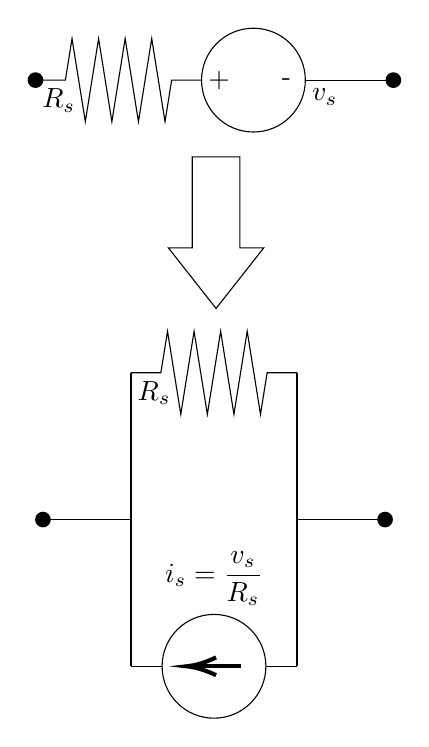
\begin{tikzpicture}[x=0.75pt,y=0.75pt,yscale=-1,xscale=1]
%uncomment if require: \path (0,420); %set diagram left start at 0, and has height of 420

%Shape: Resistor [id:dp2595676349306193] 
\draw   (201,78) -- (215.4,78) -- (218.6,58) -- (225,98) -- (231.4,58) -- (237.8,98) -- (244.2,58) -- (250.6,98) -- (257,58) -- (263.4,98) -- (266.6,78) -- (281,78) ;
%Shape: Circle [id:dp4726702298609462] 
\draw   (281,78) .. controls (281,64.19) and (292.19,53) .. (306,53) .. controls (319.81,53) and (331,64.19) .. (331,78) .. controls (331,91.81) and (319.81,103) .. (306,103) .. controls (292.19,103) and (281,91.81) .. (281,78) -- cycle ;
%Down Arrow [id:dp4867236113743594] 
\draw   (265,158.8) -- (276.5,158.8) -- (276.5,115) -- (299.5,115) -- (299.5,158.8) -- (311,158.8) -- (288,188) -- cycle ;
%Shape: Circle [id:dp48521310032792564] 
\draw   (262,360.42) .. controls (262,346.61) and (273.19,335.42) .. (287,335.42) .. controls (300.81,335.42) and (312,346.61) .. (312,360.42) .. controls (312,374.23) and (300.81,385.42) .. (287,385.42) .. controls (273.19,385.42) and (262,374.23) .. (262,360.42) -- cycle ;
%Shape: Resistor [id:dp3495898000470645] 
\draw   (247,219) -- (261.4,219) -- (264.6,199) -- (271,239) -- (277.4,199) -- (283.8,239) -- (290.2,199) -- (296.6,239) -- (303,199) -- (309.4,239) -- (312.6,219) -- (327,219) ;
%Straight Lines [id:da9040938616421672] 
\draw    (247,219) -- (247,360.42) ;
%Straight Lines [id:da4086292990449345] 
\draw    (327,219) -- (327,360.42) ;
%Straight Lines [id:da5862555045777795] 
\draw    (247,360.42) -- (262,360.42) ;
%Straight Lines [id:da15193750488345903] 
\draw    (312,360.42) -- (327,360.42) ;
%Straight Lines [id:da15177579242535977] 
\draw [line width=1.5]    (300.21,360.42) -- (276.79,360.42) ;
\draw [shift={(273.79,360.42)}, rotate = 360] [color={rgb, 255:red, 0; green, 0; blue, 0 }  ][line width=1.5]    (14.21,-4.28) .. controls (9.04,-1.82) and (4.3,-0.39) .. (0,0) .. controls (4.3,0.39) and (9.04,1.82) .. (14.21,4.28)   ;
%Straight Lines [id:da8073486658814548] 
\draw    (247,289.71) -- (204.58,289.71) ;
%Straight Lines [id:da22200817290111585] 
\draw    (369.42,289.71) -- (327,289.71) ;
%Straight Lines [id:da058000108714057586] 
\draw    (373.42,78) -- (331,78) ;
%Shape: Circle [id:dp5370808686044426] 
\draw  [fill={rgb, 255:red, 0; green, 0; blue, 0 }  ,fill opacity=1 ] (369.92,78) .. controls (369.92,76.07) and (371.49,74.5) .. (373.42,74.5) .. controls (375.35,74.5) and (376.92,76.07) .. (376.92,78) .. controls (376.92,79.93) and (375.35,81.5) .. (373.42,81.5) .. controls (371.49,81.5) and (369.92,79.93) .. (369.92,78) -- cycle ;
%Shape: Circle [id:dp007409916066804634] 
\draw  [fill={rgb, 255:red, 0; green, 0; blue, 0 }  ,fill opacity=1 ] (197.5,78) .. controls (197.5,76.07) and (199.07,74.5) .. (201,74.5) .. controls (202.93,74.5) and (204.5,76.07) .. (204.5,78) .. controls (204.5,79.93) and (202.93,81.5) .. (201,81.5) .. controls (199.07,81.5) and (197.5,79.93) .. (197.5,78) -- cycle ;
%Shape: Circle [id:dp3406177813870317] 
\draw  [fill={rgb, 255:red, 0; green, 0; blue, 0 }  ,fill opacity=1 ] (365.92,289.71) .. controls (365.92,287.78) and (367.49,286.21) .. (369.42,286.21) .. controls (371.35,286.21) and (372.92,287.78) .. (372.92,289.71) .. controls (372.92,291.64) and (371.35,293.21) .. (369.42,293.21) .. controls (367.49,293.21) and (365.92,291.64) .. (365.92,289.71) -- cycle ;
%Shape: Circle [id:dp3296743674365008] 
\draw  [fill={rgb, 255:red, 0; green, 0; blue, 0 }  ,fill opacity=1 ] (201.08,289.71) .. controls (201.08,287.78) and (202.65,286.21) .. (204.58,286.21) .. controls (206.51,286.21) and (208.08,287.78) .. (208.08,289.71) .. controls (208.08,291.64) and (206.51,293.21) .. (204.58,293.21) .. controls (202.65,293.21) and (201.08,291.64) .. (201.08,289.71) -- cycle ;

% Text Node
\draw (203,81) node [anchor=north west][inner sep=0.75pt]   [align=left] {$\displaystyle R_{s}$};
% Text Node
\draw (333,81) node [anchor=north west][inner sep=0.75pt]   [align=left] {$\displaystyle v_{s}$};
% Text Node
\draw (283,78) node [anchor=west] [inner sep=0.75pt]   [align=left] {+};
% Text Node
\draw (329,78) node [anchor=east] [inner sep=0.75pt]   [align=left] {\begin{minipage}[lt]{8.67pt}\setlength\topsep{0pt}
\begin{center}
\mbox{-}
\end{center}

\end{minipage}};
% Text Node
\draw (249,222) node [anchor=north west][inner sep=0.75pt]   [align=left] {$\displaystyle R_{s}$};
% Text Node
\draw (287,332.42) node [anchor=south] [inner sep=0.75pt]   [align=left] {$\displaystyle i_{s} =\frac{v_{s}}{R_{s}}$};


\end{tikzpicture}

      \caption{An Equivalent Circuit Example}
      \label{fig:2}
    \end{figure}

\end{itemize}

\end{document}

